\documentclass{utitcphd_overleaf}
%% This file has version 0.98

%% NOTES

% Use front-end, not frontend or front end
% Use back-end, not backend or back end
% We aimed or we aim, before the implementation chapter?
% Twente Fire Brigade or the Twente Fire Brigade?
% Twente region or the Twente region?
% use city for gemeente, district for wijk, neighbourhood for buurt

% \usepackage{caption}

% % Caption setup
% \captionsetup{
%   justification=centering,
%   font=normalfont
% }

\usepackage{listings}
\usepackage{xcolor}
\usepackage[smartEllipses, fencedCode, hashEnumerators, hybrid]{markdown}


% Setup for listings to handle JavaScript and JSX (as part of React)
\lstdefinelanguage{JavaScript}{
  keywords={const, let, function, if, else, return, class, export, default, extends},
  morecomment=[l]{//},
  morecomment=[s]{/*}{*/},
  morestring=[b]',
  morestring=[b]"
}

\lstdefinelanguage{json}{
    basicstyle=\normalfont\ttfamily,
    numbers=left,
    numberstyle=\scriptsize,
    stepnumber=1,
    numbersep=8pt,
    showstringspaces=false,
    breaklines=true,
    frame=lines,
    string=[s]{"}{"},
    stringstyle=\color{blue},
    comment=[l]{:},
    commentstyle=\color{black},
    morestring=[b]",
    morecomment=[l]{//},
    morecomment=[s]{/*}{*/},
    morekeywords={true,false,null}
}


\lstset{
  language=JavaScript,
  backgroundcolor=\color{white},   % choose the background color
  extendedchars=true,
  basicstyle=\footnotesize\ttfamily, % the size of the fonts that are used for the code
  showstringspaces=false,           % underline spaces within strings only
  showspaces=false,                 % show spaces everywhere with underscores; overrides 'showstringspaces'
  numbers=left,                     % where to put the line-numbers; possible values are (none, left, right)
  numberstyle=\tiny\color{gray},    % style used for line-numbers
  stepnumber=1,                     % step between two line-numbers. If it's 1, each line will be numbered
  numbersep=5pt,                    % how far the line-numbers are from the code
  tabsize=2,                        % sets default tabsize to 2 spaces
  breaklines=true,                  % sets automatic line breaking
  breakatwhitespace=false,          % sets if automatic breaks should only happen at whitespace
  commentstyle=\color{gray},       % comment color
  keywordstyle=\color{blue},        % keyword color
  stringstyle=\color{red},          % string literal color
  escapeinside={\%*}{*)},           % if you want to add LaTeX within your code
  morekeywords={render, componentDidMount}  % add more keywords if you need them
}


%%%%%%%%%%%%%%%%%%%%%%%%%%%%%%%%%%%%%%%%
%% Various definitions that are NEEDED
% \newcommand{\fancyTitle}{Data Driven Risk Management For Fire Services: \\ Chimney Fire Prediction Application}
% \newcommand{\saneTitle}{Data Driven Risk Management For Fire Services: Chimney Fire Prediction Application}
\title{\texorpdfstring{Data Driven Risk Management For Fire Services\\ ---\\Chimney Fire Prediction Application}{Data Driven Risk Management For Fire Services - Chimney Fire Prediction Application}}
% \title{\texorpdfstring{\fancyTitle}{\saneTitle}}
%% In the title, separate lines with "\\" and use " --- " instead of periods or semicolons (if any)

\author{Ömer Esas}                                         %% Provide author name, format "First von Last"

\SetPromoter{prof.~dr.~P. XXXXXXX}{University of Twente}
\SetSecondPromoter{prof.~dr.~S. XXXXXXX}{University of Twente}   %% Leave name empty or provide name
\SetAssistantPromoter{dr.~A. S. XXXXXXX}{University of Twente}     %% Leave name empty or provide name
\SetCoverDesigner{}                                                 %% Leave name empty or provide name
\SetDissertationNumber{XXX}                                         %% Provide number, format "xxx"
\SetDefenceDate{XXXXX, XXXXXXX 29, XXXXX}                           %% Provide date, format "DayInWeek, Month DayNumber, Year"
\SetDefenceTime{12.00}                                              %% Provide time, format "xx.xx"
\SetUTRector{prof.~dr.~ir.~A. Veldkamp}                                                      %% Leave empty (for Brinksma) or provide name
\SetBirthDate{December 15, 1993}                                       %% Provide date, format "Month xx, 2xxx"
\SetBirthPlace{Izmir, Turkey}                                 %% Provide city, format "city, country"
\SetISBN{xxx--xx--xxx--xxxx--x}                                     %% Provide true number, with format
                                                                    %%   "xxx--xx--xxx--xxxx--x", do not leave empty
\SetISSN{xxxx--xxxx, No. xx--xxx}                                   %% Some theses are in a journal series,
                                                                    %%   format "xxxx--xxxx, No. xx--xxx", or leave empty
\SetDOI{http://dx.doi.org/10.3990//x.xxxxxxxxxxxxx}                 %% Leave empty or provide DOI (digital object identifier),
                                                                    %%   format "http://dx.doi.org/10.3990//x.xxxxxxxxxxxxx"
\SetPrintShop{ITC Printing Department}  %% Privide name of printing agency, format "agency, city, country"
\SetFunnyStuff{}                                                    %% Leave empty ... or allow for additional logos, institutes, thesis
                                                                    %%   series, whatnots, et cetera.  This will be typeset mid-way on the
                                                                    %%   first left-hand page, below the dissertation committee.

%%%%%%%%%%%%%%%%%%%%%%%%%%%%%%%%%%%%%%%%

\begin{document}
%%%%%%%%%%%%%%%%%%%%%%%%%%%%%%%%%%%%%%%%%%%%%%%%%%%%%%%%%%%%%%
%% READ THIS CAREFULLY!!
%% This file version is 0.98; it works with same version of utitcphd.cls
%%
%% This file must be included through \include{thesis_frontpages}
%% from your main thesis tex file.
%% Do not change the contents of this file, EXCEPT for those
%% sections indicated as EDIT ZONE.  Typically in those zones
%% you MUST add your specifics for the thesis.
%% Search for "EDIT ZONE" in the file below, and again, only
%% do edits within those zones!
%%%%%%%%%%%%%%%%%%%%%%%%%%%%%%%%%%%%%%%%%%%%%%%%%%%%%%%%%%%%%%

\makeatletter
\hypersetup{pdfborder=0 0 0,pdftitle={\thetitle},pdfauthor={\theauthor}}
% \hypersetup{pdfborder=0 0 0,pdftitle={\texorpdfstring{\fancyTitle}{\saneTitle}},pdfauthor={\theauthor}}
%%%%%%%%%%%%%%%%%%%%%%%%%%%%%%%%%%%%%%%%%%%%%%%%%%%%%%%%%%%%%%
%% FIRST TITLE PAGE
%%%%%%%%%%%%%%%%%%%%%%%%%%%%%%%%%%%%%%%%%%%%%%%%%%%%%%%%%%%%%%
\pagenumbering{alph}

\thispagestyle{empty}
{\Huge
\begin{center}

\textbf{\thetitle}\\[18mm]

\theauthor
\end{center}
}
\clearpage

%%%%%%%%%%%%%%%%%%%%%%%%%%%%%%%%%%%%%%%%%%%%%%%%%%%%%%%%%%%%%%
%% TITLE BACKPAGE
%%%%%%%%%%%%%%%%%%%%%%%%%%%%%%%%%%%%%%%%%%%%%%%%%%%%%%%%%%%%%%

\thispagestyle{empty}

\cleardoublepage

%%%%%%%%%%%%%%%%%%%%%%%%%%%%%%%%%%%%%%%%%%%%%%%%%%%%%%%%%%%%%%
%% OFFICIAL PAGE
%%%%%%%%%%%%%%%%%%%%%%%%%%%%%%%%%%%%%%%%%%%%%%%%%%%%%%%%%%%%%%
\thispagestyle{empty}
{\LARGE
	\begin{center}
		
		\textbf{\MakeUppercase{\thetitle}}
		
		\vfill
		
		\so{EngD Thesis}
		
		\vfill
		
		{\Large to obtain the degree of\\
            Engineering Doctorate (EngD) at the University of Twente,\\
			on the authority of the rector magnificus,\\
			\@UTRector,\\
			on account of the decision of the Doctorate Board,\\
			to be defended\\
			on \@DefenceDate\ at \@DefenceTime\\}
		
		\vfill
		
		{\Large by}
		
		\vfill
		
		{\textbf{\theauthor}\\
			born on \@BirthDate\\
			in \@PlaceofBirth}
	\end{center}
}
\clearpage

%%%%%%%%%%%%%%%%%%%%%%%%%%%%%%%%%%%%%%%%%%%%%%%%%%%%%%%%%%%%%%
%% APPRVOVAL AND (C) PAGE
%%%%%%%%%%%%%%%%%%%%%%%%%%%%%%%%%%%%%%%%%%%%%%%%%%%%%%%%%%%%%%
\thispagestyle{empty}
\noindent This EngD Thesis has been approved by: \\[\baselineskip]

\noindent\@Promoter\ (promoter)\\
\ifsecondpromoter\noindent\@SecondPromoter\ (promoter) \\ \fi
\ifassistantpromoter\noindent\@AssistantPromoter\ (assistant promoter) \\ \fi
\ifsecondassistantpromoter\noindent\@SecondAssistantPromoter\ (assistant promoter) \fi

\vfill

\iffunnystuff \@FunnyStuff \fi    %% Allow for additional logos, institutes, thesis series, whatnots, et cetera.

\vfill

% \noindent ITC dissertation number \@DissertationNumber \\
% ITC, P.O. Box 217, 7500 AE Enschede, The Netherlands

{\small\vspace*{2mm}

% \begin{tabbing}
% Printed byby \= \kill
% ISBN:                    \> \@ISBN \\
% \ifissn ISSN:            \> \@ISSN \\ \fi
% \ifdoi DOI:              \> \@DOI  \\ \fi
% \ifprintshop Printed by: \> \@PrintShop \\ \fi
% \end{tabbing}

\vspace*{-2mm}  % Is 2mm minus the extra tabbing afterspace

\noindent\copyright\ \theauthor, Enschede, The Netherlands\\
\ifcoverdesigner\copyright\ Cover design by \@CoverDesigner\\ \fi
All rights reserved. No part of this publication may be reproduced without the prior written
permission of the author.

\vspace*{2mm}
}

\noindent
\includegraphics[width=\textwidth]{support/UT_logo.pdf}

\clearpage

%%%%%%%%%%%%%%%%%%%%%%%%%%%%%%%%%%%%%%%%%%%%%%%%%%%%%%%%%%%%%%

\clearpage
%%%%%%%%%%%%%%%%%%%%%%%%%%%%%%%%%%%%%%%%%%%%%%%%%%%%%%%%%%%%%%
\makeatother


\openright
\frontmatter

%-------------------------------------------------------------------------------
% Preface
%-------------------------------------------------------------------------------
% \include{Abstract}
% \include{Samenvatting}
% \include{Acknowledgments} %% Remove for review
% \include{nomenclature}

%-------------------------------------------------------------------------------
% Index
%-------------------------------------------------------------------------------
\tableofcontents

%-------------------------------------------------------------------------------
% Main Matter
%-------------------------------------------------------------------------------
\mainmatter

\chapter{Introduction}
\label{chap:introduction}


\section{Background}

TODO: Mention archimate is heavily used in this engd thesis, cite its website, briefly explain what it is.

As shown in Figure~\ref{fig:yourlabel}, ...

\begin{figure}[ht]
  \centering
  
\includegraphics[width=0.8\textwidth]{my_images/kitten.jpeg}
  \caption{Your caption text goes here}
  \label{fig:yourlabel}
\end{figure}




\section{Motivation}

In this section, the driving forces behind the need for our project and its alignment with the strategic goals of Twente Fire Brigade are explained. The collaborating parties, their goals and overarching drivers are illustrated in Figure~\ref{fig:motivation}, through the motivation elements of ArchiMate modeling framework.

\begin{figure}[ht]
  \centering
  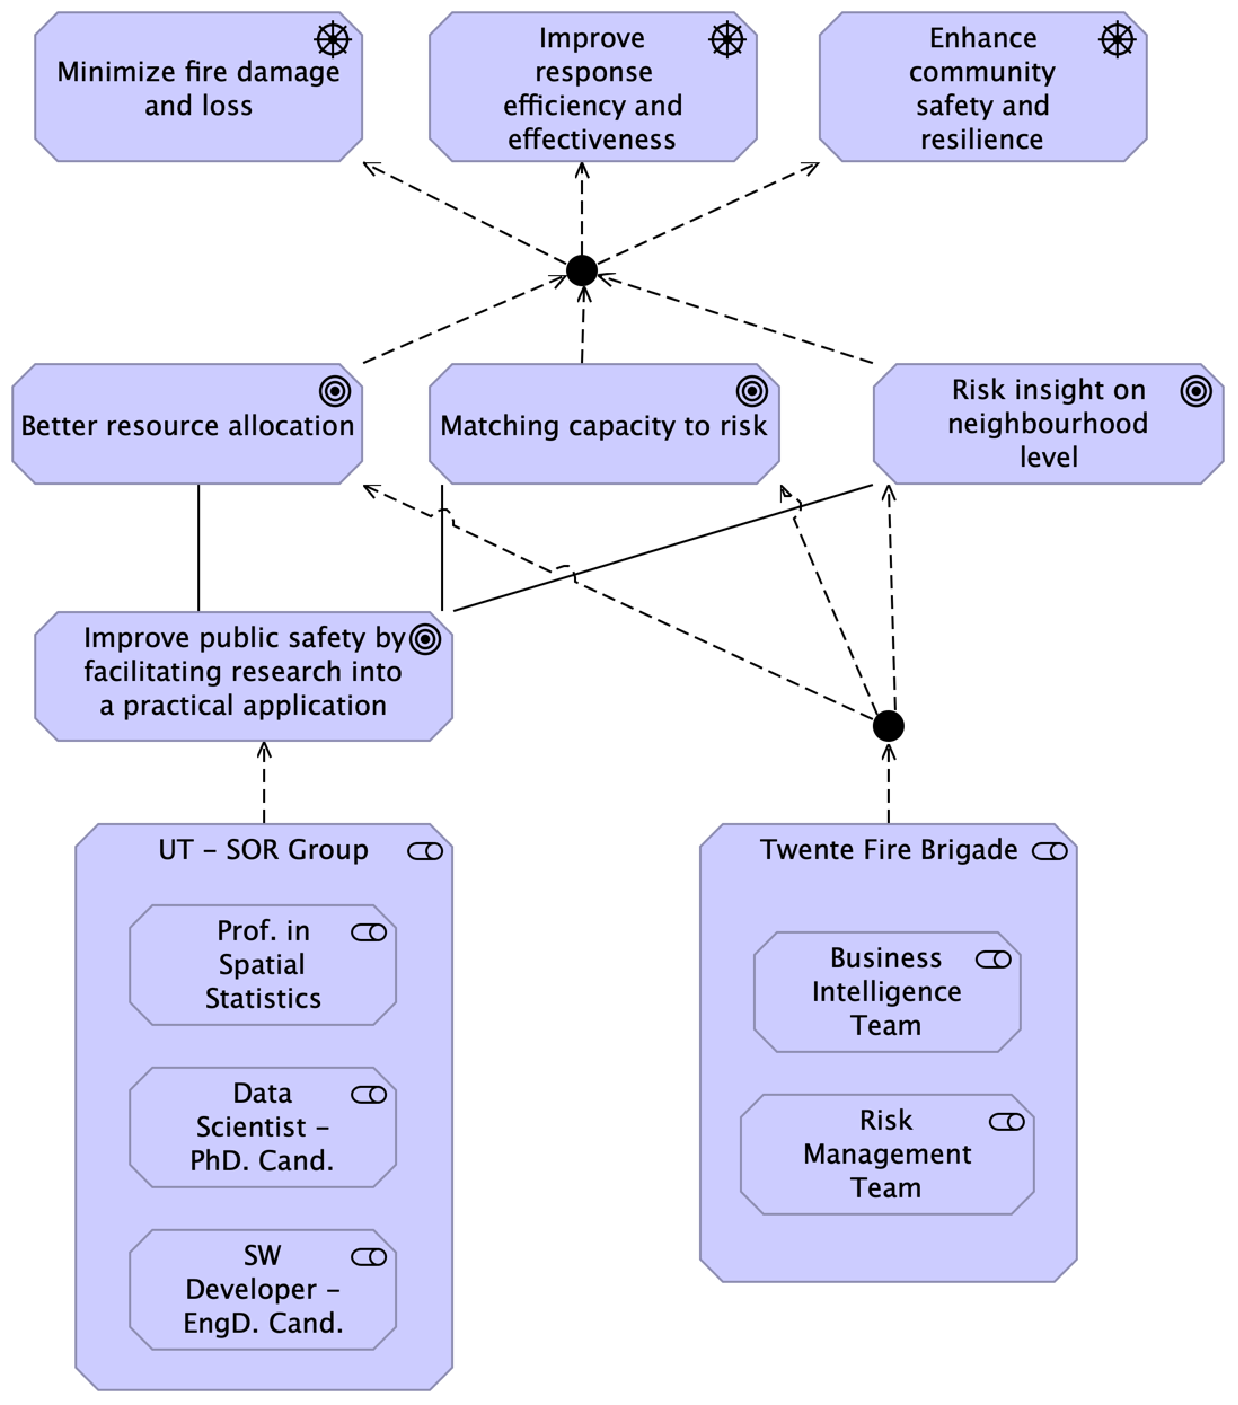
\includegraphics[width=0.8\textwidth]{my_images/other/motivation.pdf}
  \caption{Motivations Behind the Development of the Chimney Fire Prediction Application}
  \label{fig:motivation}
\end{figure}

The initial group of stakeholders comprises three members from the Stochastic Operations Research group at the University of Twente. The team is led by a professor who also serves as a senior researcher specializing in spatial statistics and acts as the project's supervisor on the university's behalf. Under her guidance are a PhD candidate and an EngD candidate, who focus on data science and software development, respectively. Collectively, our research team are eager to apply their research toward directly enhancing public safety. Their responsibilities include conducting fire risk prediction research and developing its application for the Twente Fire Brigade, which will be elaborated upon in Section \ref{sec:organization}.

From the industry side, the research conducted by the SOR group and the three stakeholders could significantly enhance the operational planning of Twente Fire Brigade. The risk management and business intelligence (BI) teams of Twente Fire Brigade are committed to leveraging their BI capabilities to gain deeper insights into chimney fire risks on a neighbourhood level. This enhanced understanding will enable them to more effectively allocate fire crews and assets, and strategically plan future resources based on the assessed risks.

The motivations illustrated in Figure~\ref{fig:motivation} reflect Twente Fire Brigade's commitment to their core mission: protecting life, property, and the environment from the devastating effects of fires and other emergencies. Eager to enhance their capabilities in minimizing fire damage and optimizing response strategies, Twente Fire Brigade aims to strengthen public safety and resilience. This collaboration with the SOR group of the University of Twente enables them to combine advanced business intelligence and academic research, thereby achieving their strategic objectives and improving their operational effectiveness.

\section{Organization}
\label{sec:organization}

The development of our sophisticated application demanded a coordinated effort involving participants of diverse backgrounds, each contributing to this endeavour from many perspectives. A detailed diagram that depicts the collaborators and their contribution is presented in Figure~\ref{fig:organization}.

\begin{figure}[ht]
  \centering
  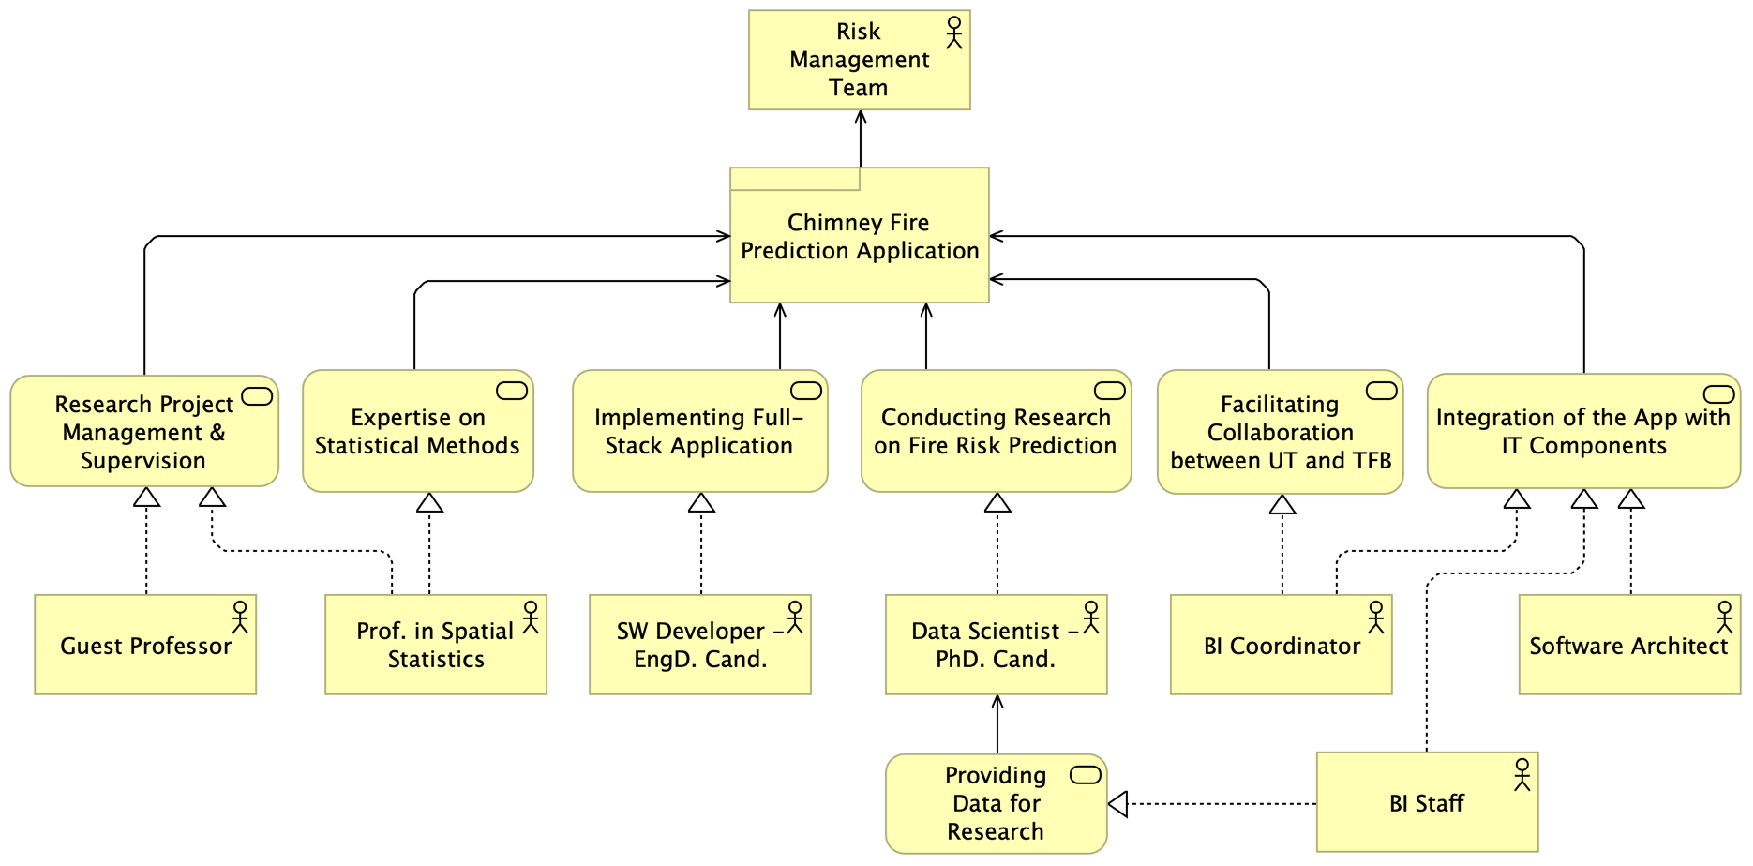
\includegraphics[width=1\textwidth]{my_images/other/organization.pdf}
  \caption{Collaborators and Their Contributions to the Chimney Fire Prediction Application}
  \label{fig:organization}
\end{figure}

At the core of our project is the foundational research conducted by the PhD candidate, which was crucial for facilitating the subsequent design and implementation of our chimney fire prediction application. Under the mentorship of two professors specializing in mathematical modeling ??? and spatial statistics, the PhD candidate developed a mathematical model that is able to predict the chimney fire risk intensity, by integrating machine learning and spatial statistics methods. The predictive model was trained on datasets comprising past chimney fire incident records and various spatio-temporal data, provided by the business intelligence staff of Twente Fire Brigade. The successful output of this research paved the way for transitioning into the implementation phase of our application.

Continuing from the research output, I, as the EngD candidate, took the lead in the application development, focusing on translating the predictive models into a practical software solution for the Twente Fire Brigade. This responsibility involved the design and implementation of a robust software architecture capable of providing accurate predictions of chimney fire risks to the risk management team.

The professors, with extensive experience in managing research projects, oversaw the whole project, making sure that all activities adhered to high standards and the objectives of the project are met. Meanwhile, the BI coordinator played a pivotal role in fostering effective collaboration between the academic staff, the business intelligence and the risk management teams of Twente Fire Brigade. Furthermore, between the development iterations, the software architect facilitated the deployment and integration of our application.

Together, these efforts from different actors highlight the importance of collaboration and interdisciplinary skills in tackling complex projects. This project not only helps the risk management team for operational planning tasks but also serves as a modal for future collaborations between academia and public safety organizations.

\section{Outline of the EngD Thesis}


\chapter{Problem Investigation}
\label{chap:problem}

\section{Mathematical Model Analysis}

\begin{figure}[ht]
  \centering
  
\includegraphics[width=0.8\textwidth]{my_images/kitten.jpeg}
  \caption{Algorithm (variable importance etc) in Archi Already}
  \label{fig:yourlabel}
\end{figure}

\begin{figure}[ht]
  \centering
  
\includegraphics[width=0.8\textwidth]{my_images/kitten.jpeg}
  \caption{Risk Map (R Plot)}
  \label{fig:yourlabel}
\end{figure}


\section{IT Systems of Twente Fire Brigade}

\begin{figure}[ht]
  \centering
  
\includegraphics[width=0.8\textwidth]{my_images/kitten.jpeg}
  \caption{IT Landscape (Backend, where data comes from) of TFB in Archi Already}
  \label{fig:yourlabel}
\end{figure}


\begin{figure}[ht]
  \centering
  
\includegraphics[width=0.8\textwidth]{my_images/kitten.jpeg}
  \caption{IT Landscape (Frontend) of TFB in Archi Already}
  \label{fig:yourlabel}
\end{figure}

\chapter{Methodology}
\label{chap:management}


\section{Design Approach}

TODO: Mention why agile

\section{Architectural Design of Milestones}

\subsection{Milestone 1}

In the design phase of Milestone 1, our goal was to quickly establish a functioning software tool that relied on historical data for its predictions. By the conclusion of this milestone, we aimed to have a backend API capable of forecasting chimney fire risks across various areas of the Twente region using the past weather data. Even though employing historical data compromises the accuracy of our predictions, it simplifies the implementation and allows us to quickly integrate and test the IT systems, ensuring all components operate smoothly and validate the system's overall functionality from the outset. This ensures all components are able to function as expected right from the start and establishes a reliable basis for the features planned in subsequent milestones. With this mindset, we designed the architecture of Milestone 1 to consist of a simple API and the necessary IT systems from Twente Fire Brigade for visualization purposes, as seen in Figure~\ref{fig:iteration_1_arch}.

\begin{figure}[ht]
  \centering
  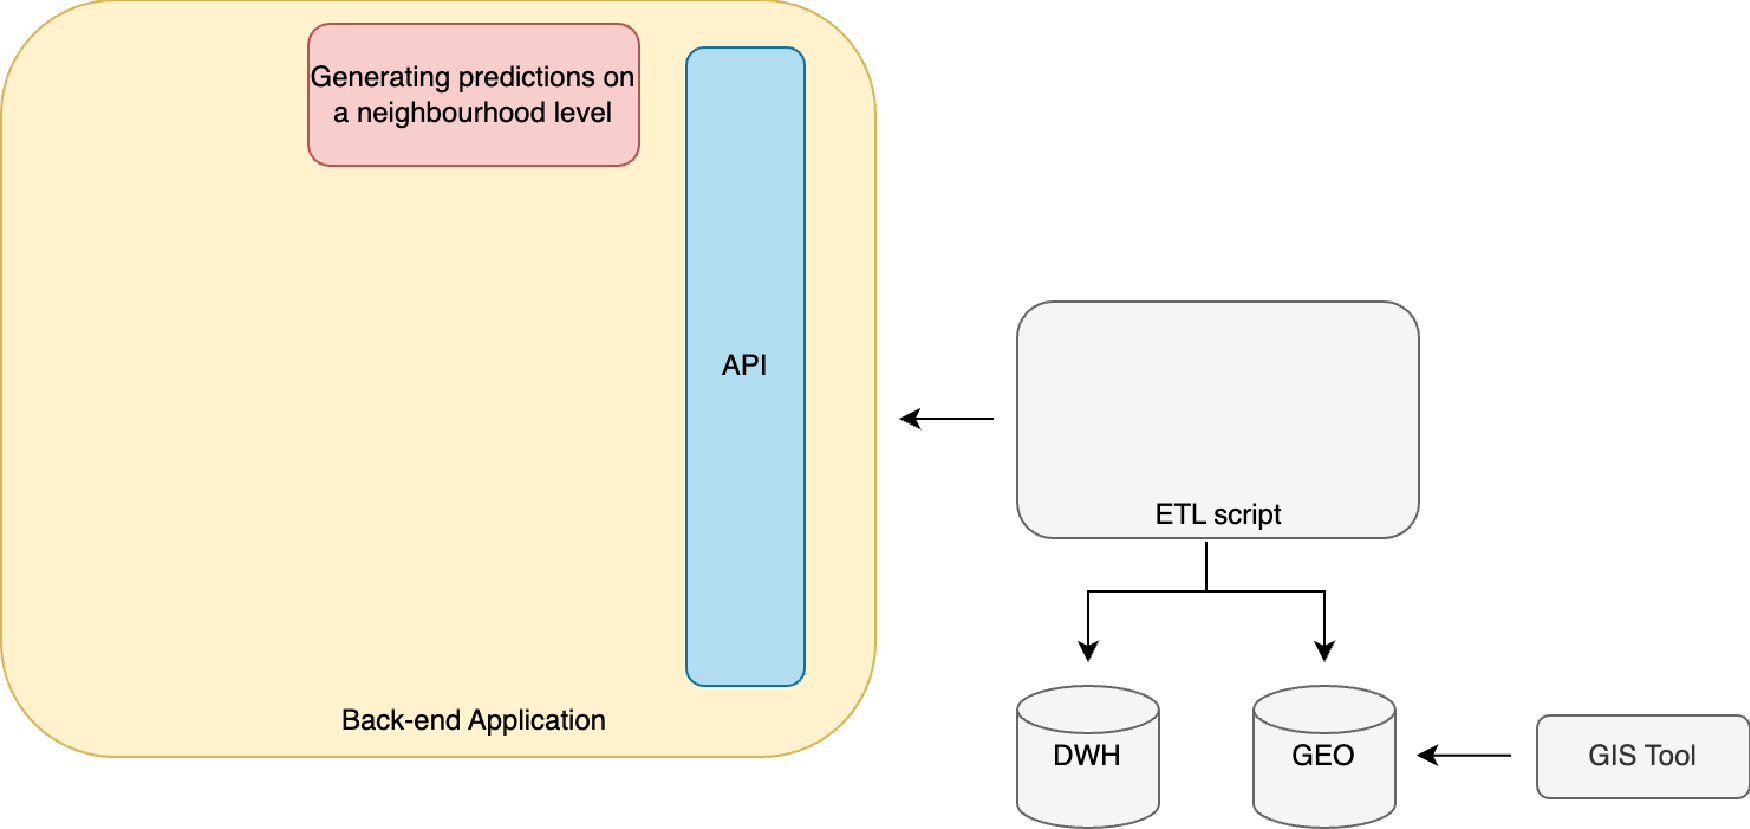
\includegraphics[width=1\textwidth]{my_images/milestones/iteration_1_arch.pdf}
  \caption{Architectural Diagram of Milestone 1}
  \label{fig:iteration_1_arch}
\end{figure}

The backend API is designed to serve as a source for generating predictions based on historical data. To fetch the chimney fire prediction data, Twente Fire Brigade is to develop an Extract-Transform-Load (ETL) script that makes HTTP GET requests to the API and saves the prediction data to the data warehouse of Twente Fire Brigade. To display the predictions on an interactive map, a Geo-Information-System (GIS) tool, which is already utilised for visualization tasks at Twente Fire Brigade as can be seen in Figure~\ref{fig:iteration_1_gis}, can connect to the data warehouse and the geo database to obtain the chimney fire prediction data and geographical information of the areas in the Twente region, respectively. Last but not least, to realise this and subsequent architectures, the application is to be deployed to Azure cloud platform in a Docker container, using the Azure account of Twente Fire Brigade.

\begin{figure}[ht]
  \centering
  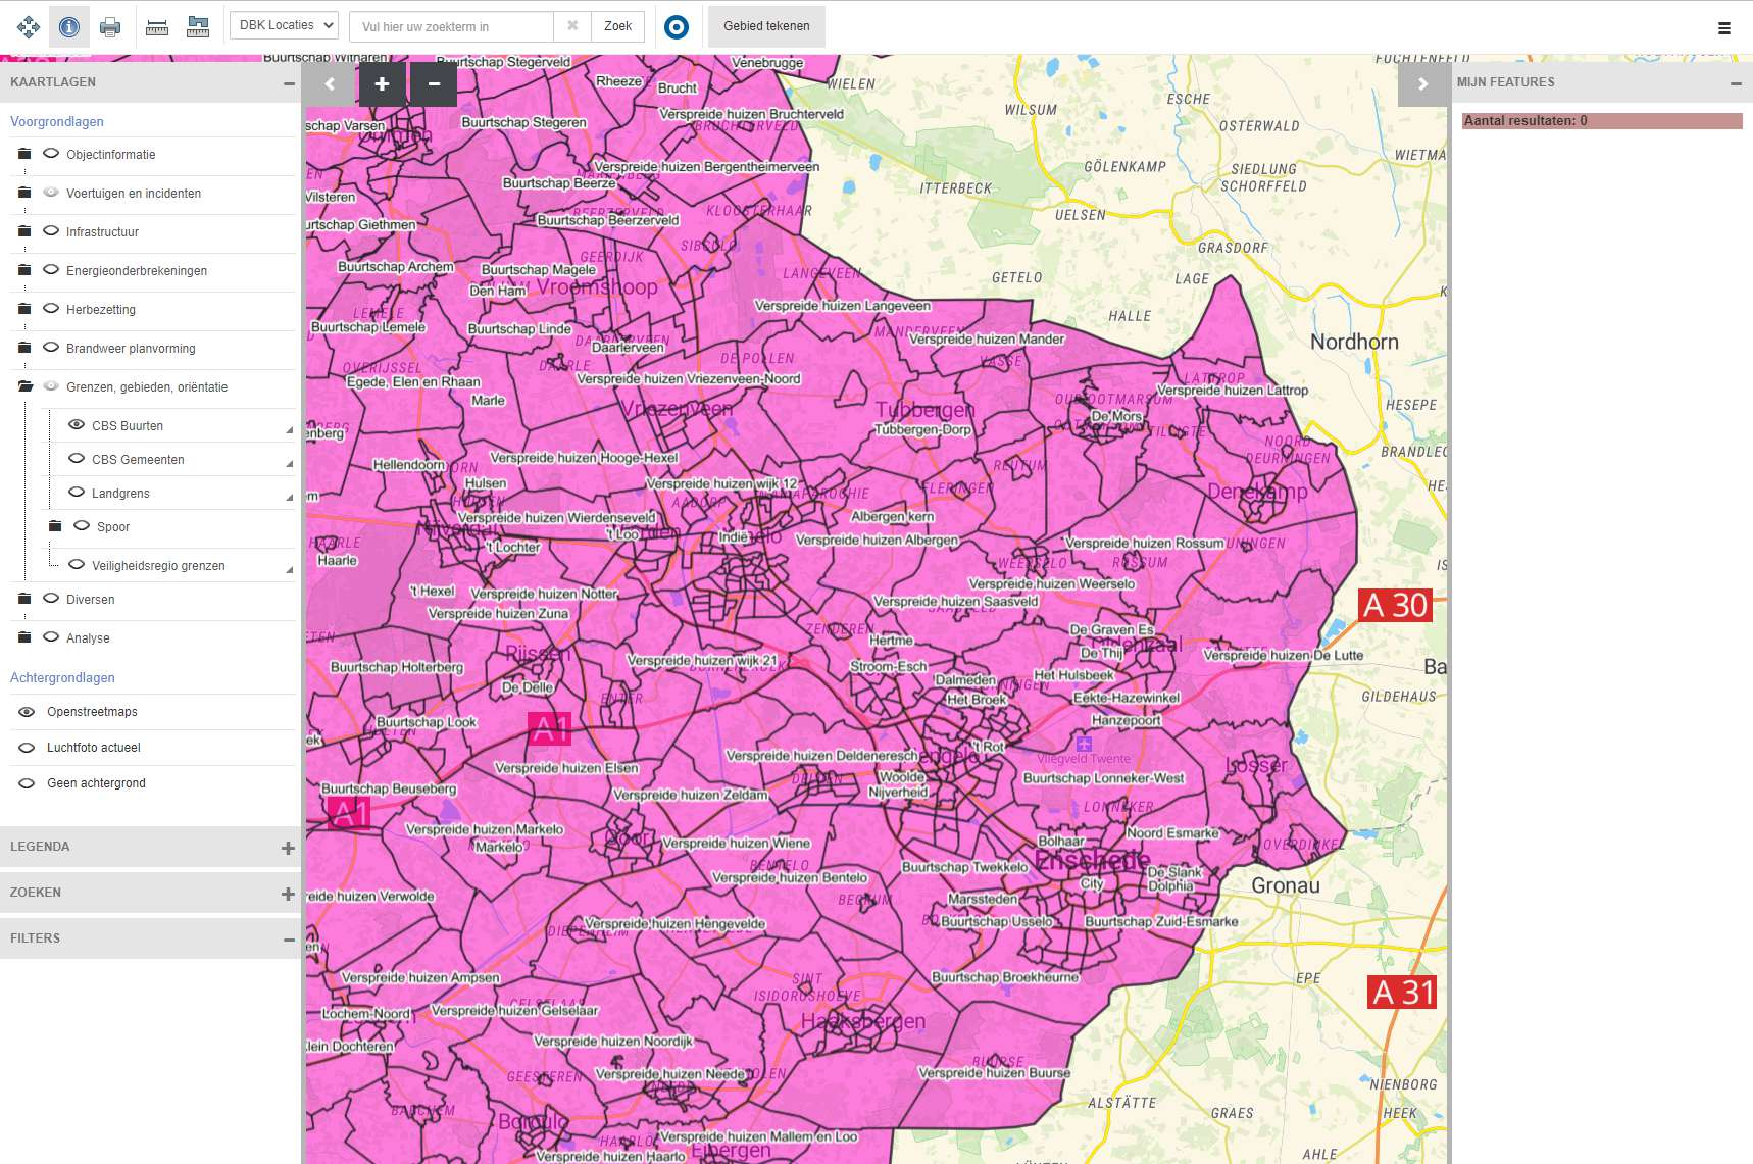
\includegraphics[width=1\textwidth]{my_images/milestones/iteration_1_gis.pdf}
  \caption{Screenshot of the GIS tool at Twente Fire Brigade}
  \label{fig:iteration_1_gis}
\end{figure}

\subsection{Milestone 2}

Building upon the solid foundation established in Milestone 1, Milestone 2 of the chimney fire risk prediction application significantly enhances both the depth and the reliability of our predictions. In this iteration, we integrate the capability to receive and process the up-to-date weather forecast data, which allows the backend application to generate more accurate and timely predictions about the chimney fire risks in the Twente region. The architectural diagram of Milestone 2 is illustrated in Figure~\ref{fig:iteration_2_arch}.

\begin{figure}[ht]
  \centering
  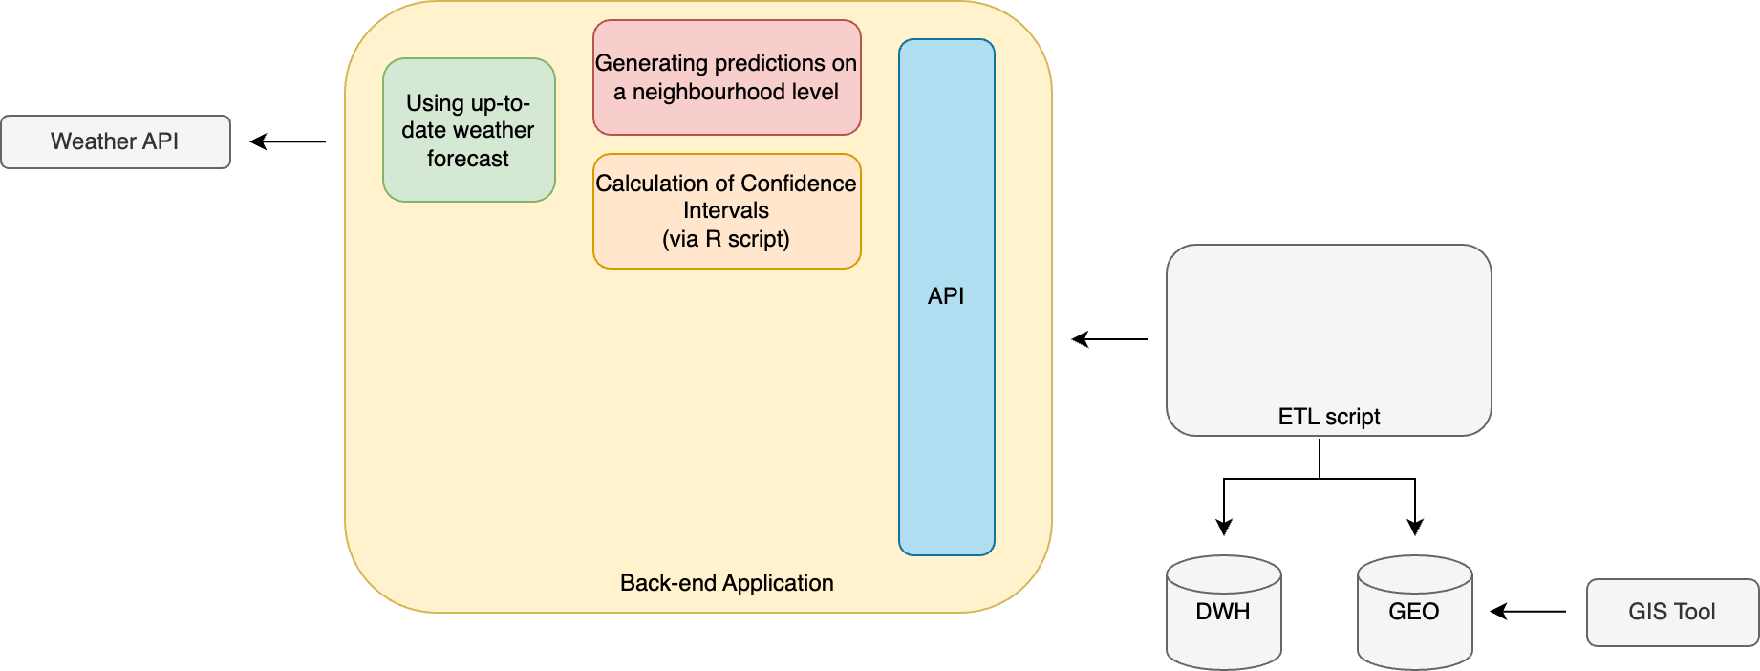
\includegraphics[width=1\textwidth]{my_images/milestones/iteration_2_arch.pdf}
  \caption{Architectural Diagram of Milestone 2}
  \label{fig:iteration_2_arch}
\end{figure}

Specifically, the backend API in Milestone 2 connects to an external weather forecasting service to obtain the up-to-date weather predictions. These forecasts include critical weather parameters that significantly influence chimney fire occurrences, such as air temperature, wind speed and the wind chill data which is derived from these two values. By incorporating current weather data, the API can adjust its risk assessments on a daily basis to reflect changing environmental conditions, thereby providing predictions that are not only based on historical weather patterns but also on the present weather scenario.

Another significant enhancement in Milestone 2 is the introduction of confidence intervals in the prediction outputs. Confidence intervals provide a statistical range that is likely to contain the true value of the number of chimney fires expected, offering an additional layer of information about the reliability and precision of the predictions. This feature is particularly valuable as it helps the decision-makers at the Twente Fire Brigade understand the uncertainty associated with the predictions, aiding them in risk assessment and resource allocation more effectively. As a side note, during the design phase of milestones, we expected that the calculation of confidence intervals might require the use of spatial statistics libraries in R, necessitating the running of some R processes in the backend application. However, this anticipation turned out to be unnecessary, as we realised in the implementation phase of Milestone 2 that Javascript is sufficient to implement the necessary mathematical algorithm, which we explained in more detail in Section \ref{sec:milestone_2}.

In short, Milestone 2 marks a significant step forward in our project, moving from a prototype that provided basic predictions based on historical data to a more sophisticated tool that utilizes up-to-date weather data and confidence intervals to enhance the prediction accuracy and utility.

\subsection{Milestone 3}

After integrating the real-time weather data and confidence intervals into our chimney fire risk prediction tool, our goal shifts towards enhancing the adaptability and the user experience of the application. To address these objectives, we structured the necessary work into two distinct stages, to be implemented in Milestone 3 and Milestone 4. In Milestone 3, we AIM/AIMED ??? to implement the application's backend logic that recalculates the parameters of the mathematical model, in addition to developing a user-friendly frontend application. The architectural diagram of Milestone 3 is presented in Figure~\ref{fig:iteration_3_arch}.

\begin{figure}[ht]
  \centering
  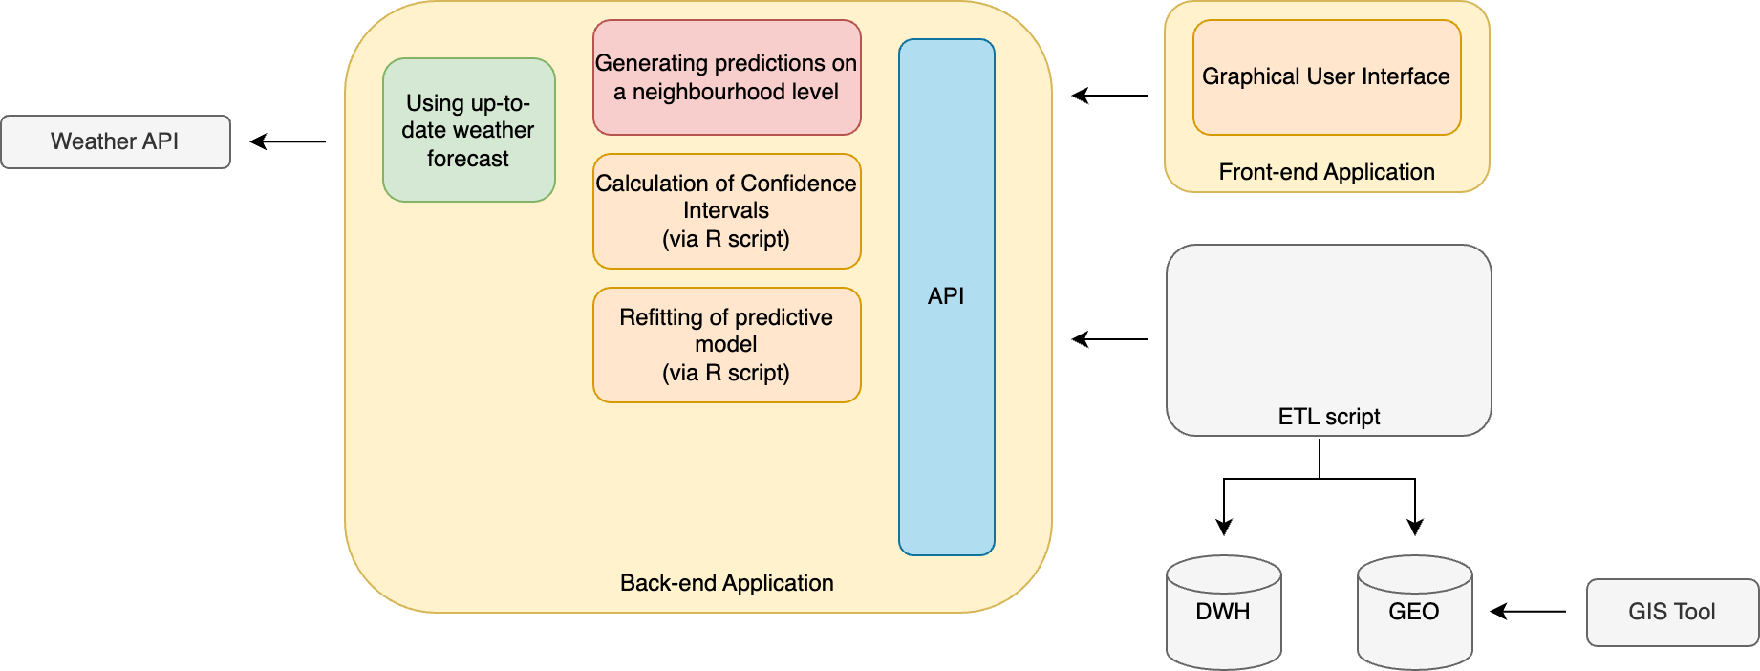
\includegraphics[width=1\textwidth]{my_images/milestones/iteration_3_arch.pdf}
  \caption{Architectural Diagram of Milestone 3}
  \label{fig:iteration_3_arch}
\end{figure}

The first feature of Milestone 3 is to realise the capability of refitting the model parameters, specifically, the coefficients of the temporal term of the mathematical model, by means of executing an R script that includes appropriate spatial statistics and linear model libraries. To ease the implementation efforts, our goal in Milestone 3 IS/WAS ??? to achieve the correct application logic, using the same dataset that is initially used to fit the model parameters. Even though employing the same dataset in the model training process would result in very similar coefficients compared to existing model parameters, hence not make the application any more accurate in terms of predictions, this would ensure the effectiveness and the correct behaviour of the model refitting mechanism and act as a precursor to using new training data in Milestone 4.

In addition to the efforts in making sure the application would stay relevant, we also aimed to develop a front-end application that serves as a graphical user interface for the users at Twente Fire Brigade. This would enhance the user interaction with the application, enabling the users to trigger the model fitting process, without the need to have the IT skills to interact with the back-end application via manual HTTP requests.

In summary, our goals in Milestone 3 were to lay the groundwork for increased adaptability and the user experience of our chimney fire risk prediction tool. By implementing the back-end logic to allow for recalibration of model parameters, we aimed to realise an essential part in providing a software tool to Twente Fire Brigade that would remain relevant in the coming years. Furthermore, the introduction of the front-end application was designed to provide user-friendly access to more sophisticated features not available through the GIS tool at Twente Fire Brigade, such as model refitting.

\subsection{Milestone 4}

In Milestone 4, we continued to build on the groundwork laid in Milestone 3, with a particular emphasis on finalizing the model refitting feature. By implementing a mechanism that allows users to input new datasets into the application, we aimed to fully harness the adaptability of the mathematical model. This enhancement ensures that the Twente Fire Brigade can utilize the most current and relevant data, thereby maximizing the benefits offered by our chimney fire prediction application. The architectural diagram designed to facilitate this functionality is presented in Figure~\ref{fig:iteration_4_arch}.

\begin{figure}[ht]
  \centering
  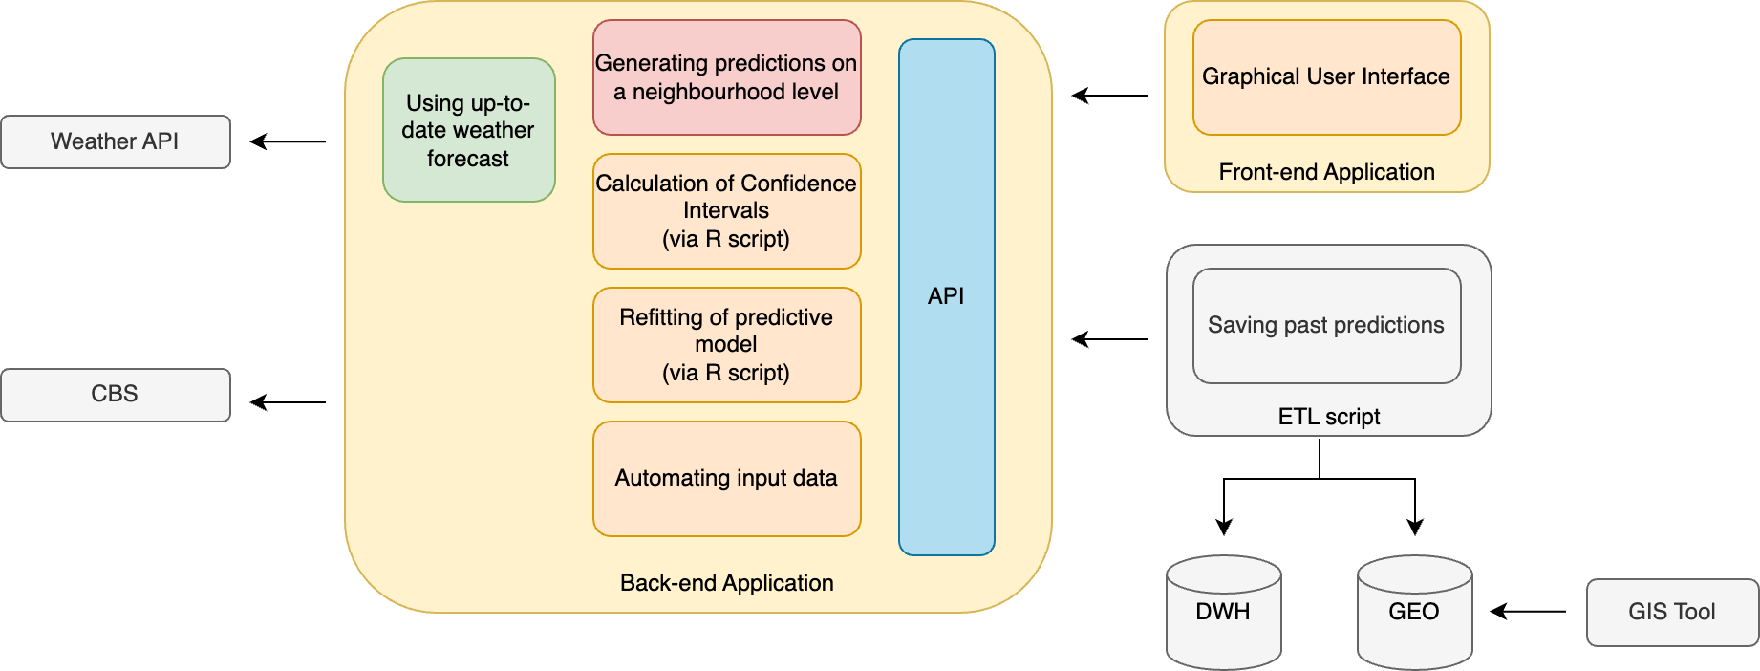
\includegraphics[width=1\textwidth]{my_images/milestones/iteration_4_arch.pdf}
  \caption{Architectural Diagram of Milestone 4}
  \label{fig:iteration_4_arch}
\end{figure}

The key feature of Milestone 4 is the capability of the back-end application to receive and process new input data for training the predictive model. This process can be initiated on-demand via the front-end application, enabling users at the Twente Fire Brigade to trigger the retraining process as needed. The retraining involves updating the model's coefficients based on the latest data, which not only refines its predictions but also adapts to any changes in spatio-temporal factors affecting chimney fire risks.

During the design phase of Milestone 4, as illustrated in Figure~\ref{fig:iteration_4_arch}, we designed our architecture under the assumption that we would be able to identify and integrate an appropriate data source, such as CBS, into our application. However, not all necessary input data might be readily accessible via APIs. The retrieval, reformatting and integration of these new datasets might require thorough investigation and the development of new ETL (Extract, Transform, Load) processes within our back-end application. This might involve complex data cleansing and preparation steps to ensure that the data fed into the model is clean, relevant and structured appropriately.

Additionally, as part of Milestone 4, we wanted to illustrate that Twente Fire Brigade can explore further enhancements and discover new ways to benefit from our chimney fire prediction application. For example, they can implement changes to their ETL processes to save these predictions after they receive the daily chimney fire risk data. This stored data can then be used to compare the predicted risk levels with the actual occurrences of chimney fire incidents. Such comparisons not only validate the accuracy of the predictions but also provide critical feedback that can be used to refine the predictive model. This process enhances its effectiveness and reliability over time, offering substantial support to the risk management team by demonstrating the reliability of the predictions, thereby helping them gauge how much they can confidently rely on these insights for making informed decisions.

In conclusion, Milestone 4 represents the completion of our project, where we have built upon and refined the capabilities established in earlier milestones. This final stage focused on enhancing the adaptability of our predictive model through the integration of new and varied datasets in a user friendly way, enabling on-demand retraining processes that adjust the model’s parameters to reflect the latest spatio-temporal data. During the design phase of Milestone 4, the specific mechanism for inputting new data was not fully defined, and we continued under the assumption that it will become clearer and easier to assess the feasibility of various options as we progress through the implementation of the previous milestones. This iterative approach allows us to refine our strategies and ensure the most effective integration of new data into the system. All in all, these enhancements guarantee that the Twente Fire Brigade can access the most up-to-date risk data, thus optimizing the utility and efficacy of the chimney fire prediction application, allowing them to benefit from its predictions in risk management operations for many years to come.

\section{Technology Choices}

TODO why node.js, docker, node.js child process, express, JS as full stack etc

\chapter{Implementation}
\label{chap:implementation}

TODO:Mention that city=gemeeente, district=wijk, ... 

MENTION THE TECH STACK, mention example api request and responses in appendix

% \begin{lstlisting}[label={lst:listing-js}, language=JavaScript, caption=React Component Example]
% import React, { Component } from 'react';

% class App extends Component {
%   componentDidMount() {
%       // Code to run on component mount
%   }

%   render() {
%     return (
%       <div>
%         Hello, world!
%       </div>
%     );
%   }
% }

% export default App;
% \end{lstlisting}

% An example table can be seen in Listing \ref{lst:listing-js}.


\section{Implementation of Milestones}

where the application model elements from Archimate modeling language are utilized.

\subsection{Milestone 1}

As the first step in the implementation phase, to start producing the predictions and providing them to the Twente Fire Brigade, the application logic implemented is illustrated in Figure~\ref{fig:m1_logic}. To fetch the prediction data, the application is sent an API request by the ETL script, which involves the data about the day and the area of interest as query parameters. The application then validates if the query parameters are valid, in other words, if the date is a date string in proper format, such as in "2023-01-25", and if the area code is a valid CBS area code, such as “GM0153” for the city of “Enschede” or “WK015303” for the district of “Twekkelerveld” in Enschede. If both query parameters are valid, then the application calculates the predicted number of chimney fires for that area on that day. An example API GET request and response in Milestone 1 is presented in Appendix~\ref{section:appendix_milestone_1}.

\begin{figure}[ht]
  \centering
  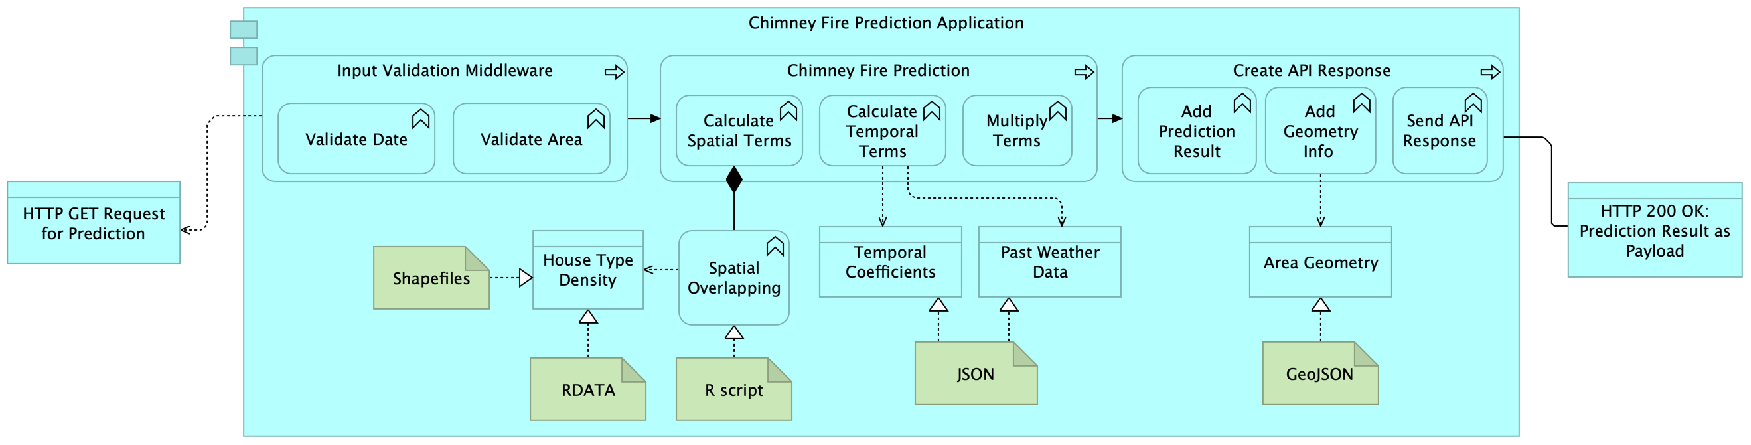
\includegraphics[width=1\textwidth]{my_images/milestones/m1.pdf}
  \caption{Application Logic of Milestone 1}
  \label{fig:m1_logic}
\end{figure}

To avoid complexity in the first milestone, we decided to simplify the prediction generation process, which consists of calculating spatial and temporal terms and multiplying them to have the actual prediction result. To have the spatial terms, we took a straightforward approach and implemented this in a similar way to the code used in the research paper of this project. More specifically, we used the density information of houses of different types in the format of “shapefile” and “.RData” objects. Then, we made use of the “spatial overlapping” functions in R to have the spatial terms for the area given as a query parameter. As for the temporal terms for that date, we utilised only the historical weather data, namely, the wind speed and wind chill values for the Twente region in 2020, which we stored as JSON files alongside the temporal coefficients used to calculate the temporal terms for the date given as a query parameter in the API request. Multiplying the calculated spatial terms for the area of interest and temporal terms for the date of interest, we have the predicted number of chimney fires for that area on that date.

The course of the API request ends with creating and sending the API response in JSON format. Finally, the geometry information of the area is included in the response, in case the API request made by the ETL script of the Twente Fire Brigade required this geometry information in GeoJSON format so that the GIS tool is able to draw the borders of the area of interest on the map of the Twente. In short, at the end of Milestone 1, we implemented the prototype which can process the API requests and respond with a prediction result, although only using historical weather data instead of up-to- date weather forecast, hence not responding with the most accurate predictions.

\subsection{Milestone 2}
\label{sec:milestone_2}

In the second milestone version of the chimney fire prediction application, we aimed to equip the application with the capability of having access to up-to-date weather forecasts, so that it uses current weather info in making predictions about the number of chimney fires in areas of interest. To this end, the application logic presented in Figure~\ref{fig:m2_logic} is implemented.

\begin{figure}[ht]
  \centering
  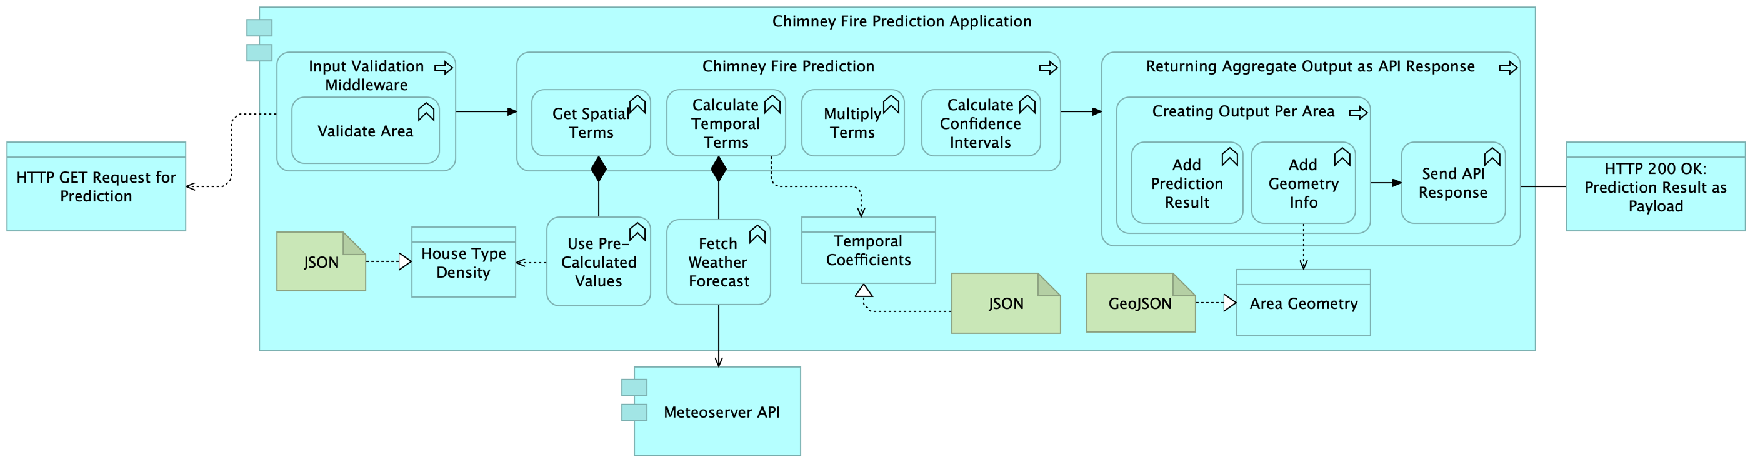
\includegraphics[width=1\textwidth]{my_images/milestones/m2.pdf}
  \caption{Application Logic of Milestone 2}
  \label{fig:m2_logic}
\end{figure}

The first major improvement in this version of the API is that it uses up-to-date weather forecasts from a weather API to calculate the temporal terms of the prediction to be made. In our implementation, we selected Meteoserver [X] as the weather forecast provider, since it uses the KNMI [X] data under the hood, which is the same data source used in the research paper of this project. The weather data is received in JSON format from the Meteoserver API, which is the native data format for Javascript-based applications. Additionally, the application is configured to receive weather data at the specific times of 0:35, 7:35, 12:35 and 18:35 every day, ensuring that the data used in making predictions is always up-to-date. One limitation of the Meteoserver API, however, is that it provides the necessary weather data, such as the average daily temperature and wind speed, only for the next ten days. Therefore, the capability of making predictions in our application is constrained by the time frame for which the weather API provides forecasts.

The second major improvement is related to the spatial terms of the prediction calculation process. Instead of using the shapefiles, R-specific objects and scripts to calculate the spatial terms each time an API request is received, we calculated the spatial terms, in other words, the number of houses of the four types defined in the mathematical model, for all Gemeente, Wijk, Buurt and 500 by 500 meter boxes in Twente region and stored the result in JSON format. Because the number of areas in the Twente region will be more or less the same in the coming years, in other words, because the number of areas will not scale as time goes on, this approach of pre-calculating and storing spatial term values for each area was reasonable and practical. Furthermore, this optimisation cut the time spent for processing API requests from approximately thirty seconds to only one second, since the compute-heavy R scripts are replaced by simple look-up operations from a JSON file via Javascript code.

The third most important change in the second milestone is the capability of returning prediction results not only on a per-area basis, but also in an aggregate way. For example, if the GIS tool or ETL script of Twente Fire Brigade would like to receive predictions for all Gemeente in Twente region, they can make an API request to the relevant endpoint, namely to “prediction/gemeente”, instead of making fourteen separate requests for fourteen different gemeente in Twente, which would be API requests to “prediction/gemeente/GM0153”, “prediction/gemeente/GM0158” and so on. In other words, in addition to the previous endpoints which return predictions per area, the second milestone version also implements four additional API endpoints: “prediction/gemeente”, “prediction/wijk”, “prediction/buurt” and “prediction/box”, which return the predictions for the areas of that type for the next ten days. Furthermore, in case the Twente Fire Brigade does not need the geospatial information of the areas of interest and would like to receive a response smaller in size, we added a query parameter "excludeGeoInfo", which can be set to "true" during the API request to omit the GeoJSON part from the response. The last change we made in the API structure in Milestone 2 is to add the "lastWeatherFetchTimestamp" property as part of API responses, which informs Twente Fire Brigade of the time the application fetched the weather forecast from the Meteoserver API. To describe these changes in the API more clearly, an example API GET request and response in Milestone 2 is illustrated in Appendix~\ref{section:appendix_milestone_2}.

During the implementation of the confidence interval calculation feature in Milestone 2, we initially considered using R scripts to manage these computations. However, upon further development, it became clear that these calculations could be effectively handled using JavaScript code exclusively. The algorithm, as illustrated in Figure~\ref{fig:m2_CI_logic}, involves several critical steps to compute the confidence intervals. First, we calculate the covariates from the wind chill and wind speed data. Next, we compute the standard deviation by multiplying these covariates with the G (Godambe) matrix, a predefined matrix that transforms the covariate data into a measure of variance. Following this, we calculate scaling factors for the upper and lower bounds of the confidence intervals. These scaling factors adjust the predictions to reflect the range within which the true values are likely to fall with 95\% confidence. Finally, we multiply the predictions with these scaling factors to derive the upper and lower bounds of the confidence intervals. These steps ensure that each prediction provided by the API now includes these bounds, allowing users to gauge the reliability and variability of the data with greater precision.

\begin{figure}[ht]
  \centering
  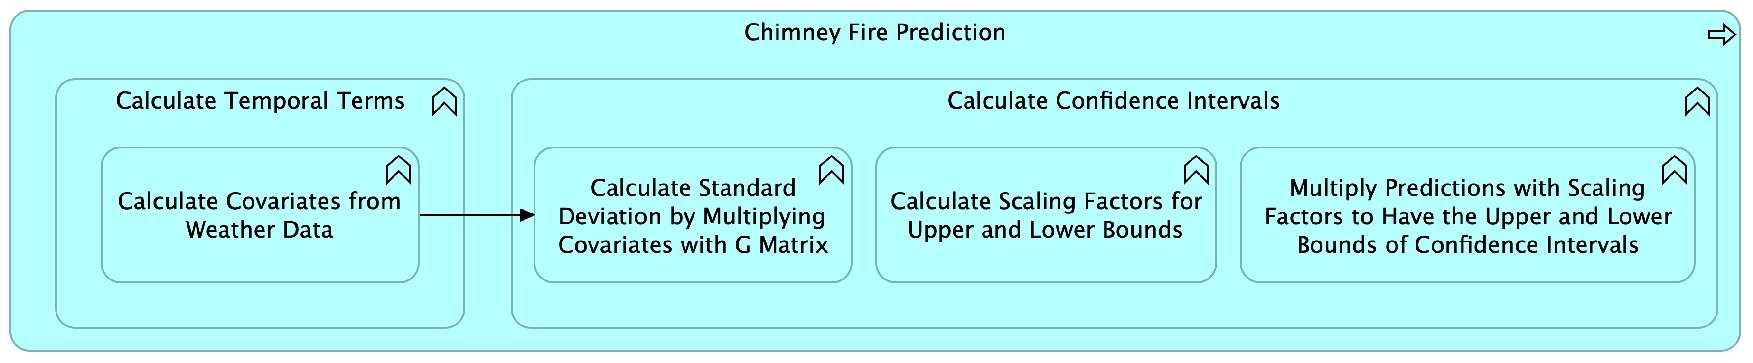
\includegraphics[width=1\textwidth]{my_images/milestones/m2_CI_logic.pdf}
  \caption{Application Logic of Confidence Interval Calculation Algorithm}
  \label{fig:m2_CI_logic}
\end{figure}

In conclusion, the second milestone of the chimney fire prediction application represents a significant advancement in our ability to provide timely and accurate predictions to the Twente Fire Brigade. By integrating real-time weather data, enhancing the efficiency of spatial data processing and improving the API's response capabilities, this milestone greatly increases the operational competence of the system. The ability to incorporate the confidence intervals further strengthens the reliability of the predictions, providing the Fire Brigade with crucial data to make informed decisions. From this milestone and onwards, the Twente Fire Brigade is able to truly reap the benefits of our chimney fire prediction tool, making it a valuable part of their risk management and operational planning processes.

\subsection{Milestone 3}

\begin{figure}[ht]
  \centering
  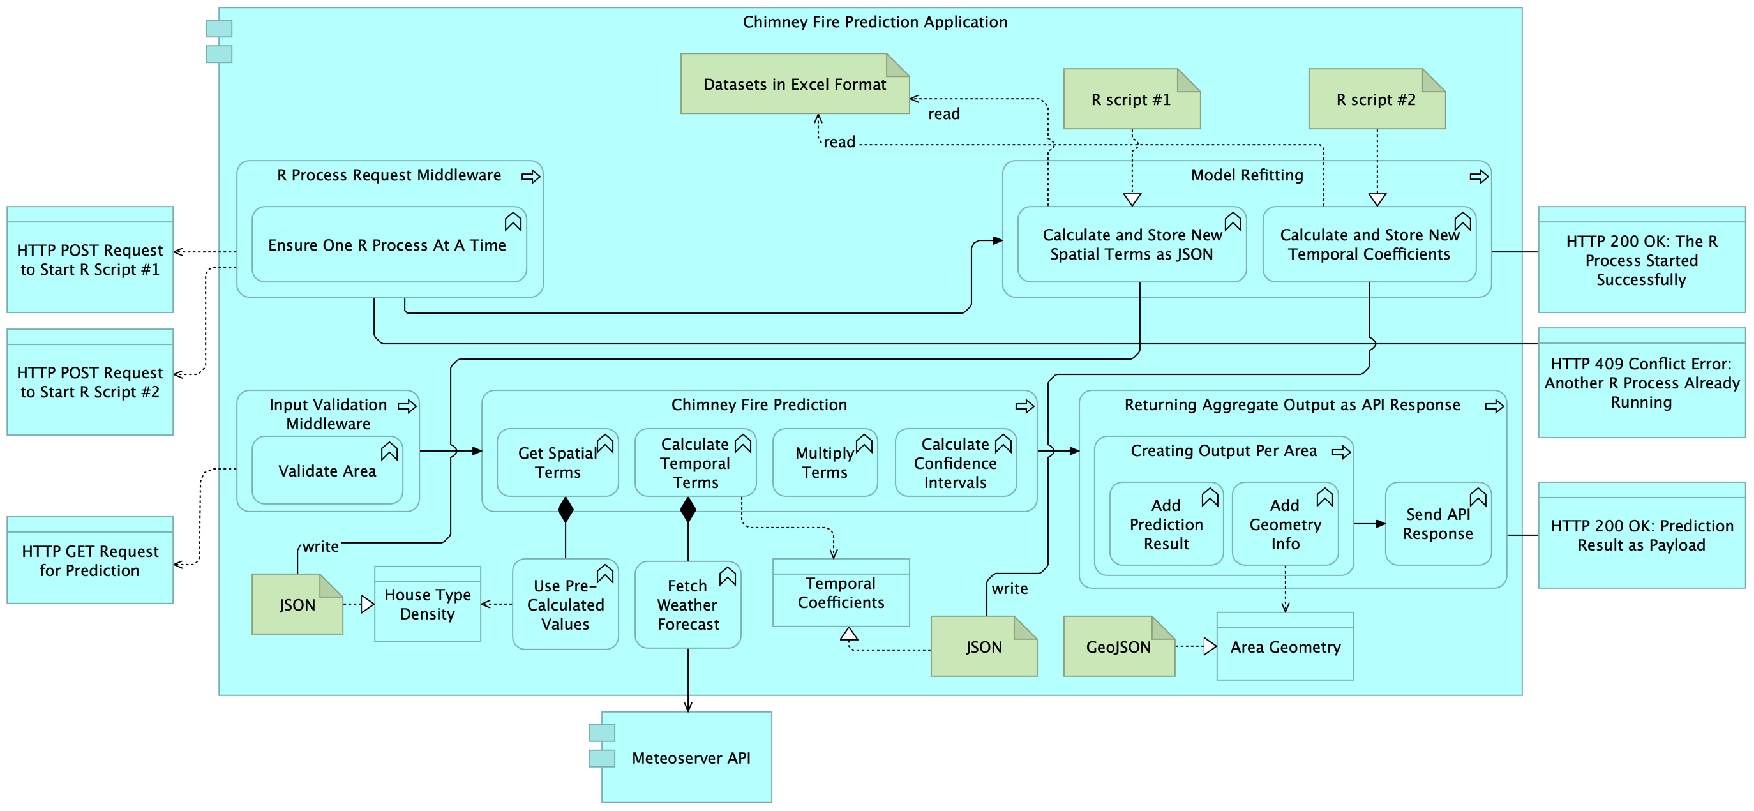
\includegraphics[width=1\textwidth]{my_images/milestones/m3-2.pdf}
  \caption{Application Logic of Milestone 3}
  \label{fig:m3_logic}
\end{figure}

\subsection{Milestone 4}

\begin{figure}[ht]
  \centering
  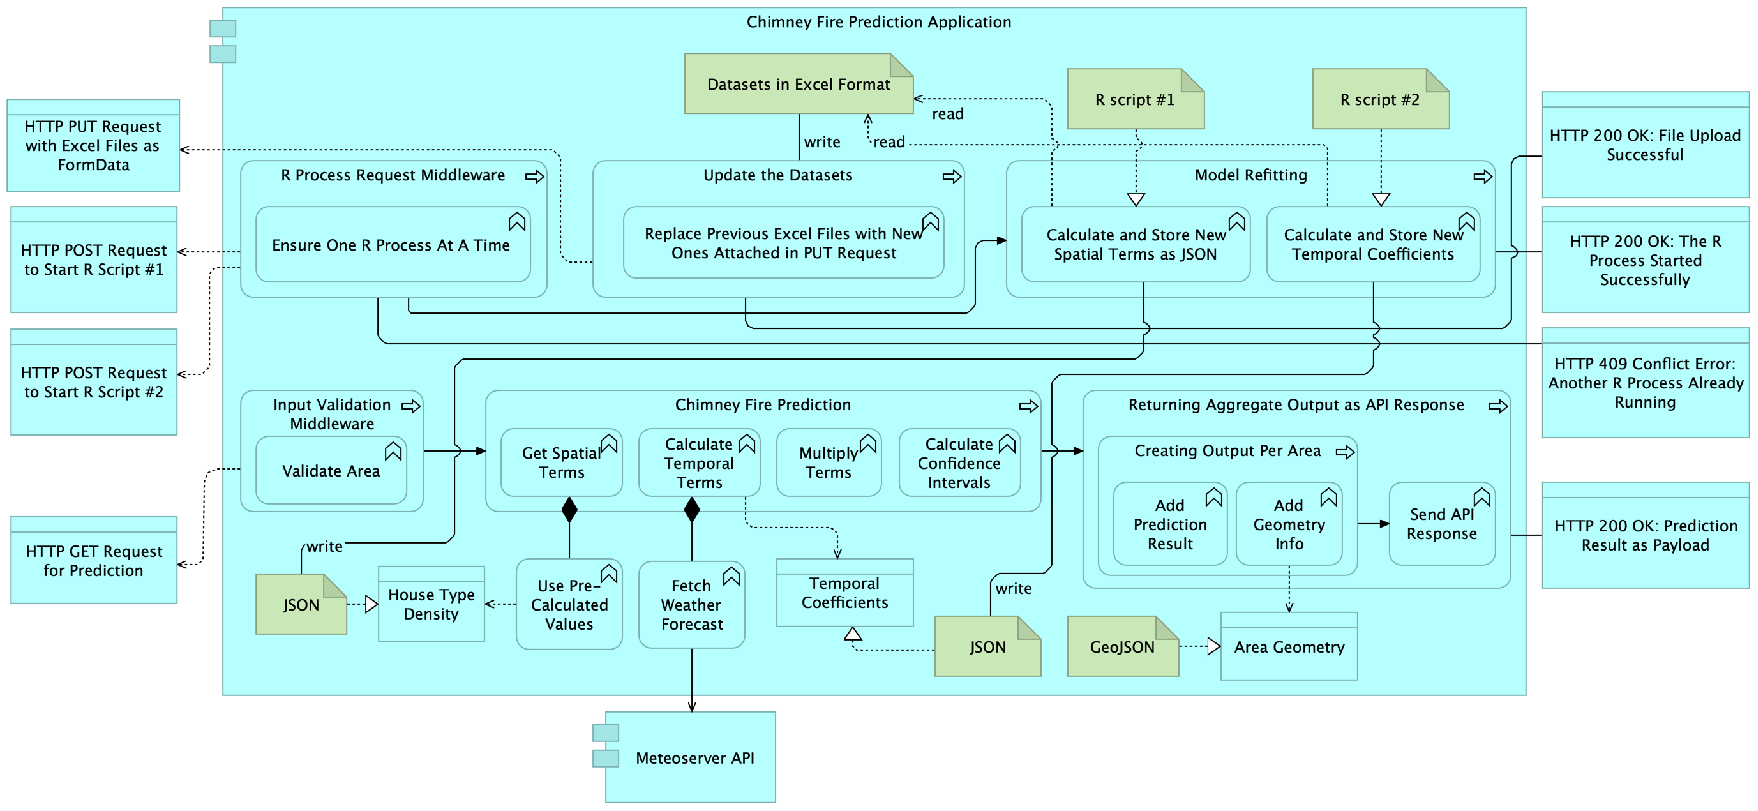
\includegraphics[width=1\textwidth]{my_images/milestones/m4.pdf}
  \caption{Application Logic of Milestone 4}
  \label{fig:m4_logic}
\end{figure}


\section{Frontend Application}

\chapter{Deployment \& Validation}
\label{chap:deployment}

\section{Deployment}

\section{Validation}


\chapter{Conclusion and Future Work}
\label{chap:conclusion}

%-------------------------------------------------------------------------------
% Appendix
%-------------------------------------------------------------------------------
\appendix
\chapter{GitHub Repository}

Here you can include additional data relevant to your thesis. This appendix is now formatted as an appendix section.

\chapter{API Endpoints}

Here you can include additional data relevant to your thesis. This appendix is now formatted as an appendix section.

\chapter{Example API Responses}

\section{Milestone 1}
\label{section:appendix_milestone_1}

An example API request and response in Milestone 1 version of the chimney fire prediction application are given in Listings \ref{lst:api_1_request} and \ref{lst:api_1_response}. Note that the array of coordinates in the "geometry" property of the API response is kept short for demonstration purposes.

\begin{lstlisting}[label={lst:api_1_request}, language=json, caption=Example API Request in Milestone 1, numbers=none]
https://chimneyfireproject.azurewebsites.net/prediction?areaCode=GM0164&date=2023-01-01
\end{lstlisting}

\begin{lstlisting}[label={lst:api_1_response}, language=json, caption=Example API Response in Milestone 1]
{
  "areaCode": "GM0164",
  "date": "2023-01-01T00:00:00.000Z",
  "predictedFires": 0.07389275859749127,
  "geoInfo": {
    "type": "Feature",
    "crs": {
      "type": "name",
      "properties": {
        "name": "urn:ogc:def:crs:EPSG::28992"
      }
    },
    "properties": {
      "id": 114,
      "fid": 114,
      "gemeenteco": "GM0164",
      "gemeentena": "Hengelo",
      "jaarstatco": "2021GM0164",
      "jaar": 2021
    },
    "geometry": {
      "type": "MultiPolygon",
      "coordinates": [
        [
          [
            [251978.591, 481220.258],
            [251979.382, 481218.495],
            [251983.707, 481220.19]
          ]
        ]
      ]
    }
  }
}
\end{lstlisting}

\section{Milestone 2}
\label{section:appendix_milestone_2}

An example API request and response in Milestone 2 version of the chimney fire prediction application are given in Listings \ref{lst:api_2_request} and \ref{lst:api_2_response}.

\begin{lstlisting}[label={lst:api_2_request}, language=json, caption=Example API Request in Milestone 2, numbers=none]
https://chimneyfireproject.azurewebsites.net/prediction/gemeente/GM0153
\end{lstlisting}

\begin{lstlisting}[label={lst:api_2_response}, language=json, caption=Example API Response in Milestone 2]
{
    "lastWeatherFetchTimestamp": "17-04-2024 15:15:13",
    "data": {
        "areaId": "GM0153",
        "prediction": [
            {
                "date": "17-04-2024",
                "numberOfFires": "0.064677",
                "lowerBoundOfFires": "0.061271",
                "upperBoundOfFires": "0.068083"
            },
            {
                "date": "18-04-2024",
                "numberOfFires": "0.063505",
                "lowerBoundOfFires": "0.060078",
                "upperBoundOfFires": "0.066931"
            },
            {
                "date": "19-04-2024",
                "numberOfFires": "0.069518",
                "lowerBoundOfFires": "0.065613",
                "upperBoundOfFires": "0.073422"
            },
            {
                "date": "20-04-2024",
                "numberOfFires": "0.081339",
                "lowerBoundOfFires": "0.076496",
                "upperBoundOfFires": "0.086181"
            },
            {
                "date": "21-04-2024",
                "numberOfFires": "0.074268",
                "lowerBoundOfFires": "0.069827",
                "upperBoundOfFires": "0.078709"
            },
            {
                "date": "22-04-2024",
                "numberOfFires": "0.086056",
                "lowerBoundOfFires": "0.080469",
                "upperBoundOfFires": "0.091644"
            },
            {
                "date": "23-04-2024",
                "numberOfFires": "0.071638",
                "lowerBoundOfFires": "0.067111",
                "upperBoundOfFires": "0.076164"
            },
            {
                "date": "24-04-2024",
                "numberOfFires": "0.058141",
                "lowerBoundOfFires": "0.054491",
                "upperBoundOfFires": "0.061790"
            },
            {
                "date": "25-04-2024",
                "numberOfFires": "0.057063",
                "lowerBoundOfFires": "0.053378",
                "upperBoundOfFires": "0.060747"
            },
            {
                "date": "26-04-2024",
                "numberOfFires": "0.067903",
                "lowerBoundOfFires": "0.063232",
                "upperBoundOfFires": "0.072574"
            },
            {
                "date": "27-04-2024",
                "numberOfFires": "0.097660",
                "lowerBoundOfFires": "0.086680",
                "upperBoundOfFires": "0.108641"
            }
        ],
        "geoInfo": {
            "type": "Feature",
            "crs": {
                "type": "name",
                "properties": {
                    "name": "urn:ogc:def:crs:EPSG::28992"
                }
            },
            "properties": {
                "id": 110,
                "fid": 110,
                "gemeenteco": "GM0153",
                "gemeentena": "Enschede",
                "jaarstatco": "2021GM0153",
                "jaar": 2021
            },
            "geometry": {
                "type": "MultiPolygon",
                "coordinates": [
                    [
                        [
                            [
                                259057.888,
                                478571.251
                            ],
                            [
                                259074.141,
                                478513.545
                            ],
                            [
                                259097.161,
                                478429.967
                            ]
                        ]
                    ]
                ]
            }
        }
    }
}
\end{lstlisting}

\chapter{Screenshots of the Frontend Application}
\label{app:additionaldata}



\listoffigures
\listoftables

%-------------------------------------------------------------------------------
% Bibliography
%-------------------------------------------------------------------------------
\bibliographystyle{abbrv}
\bibliography{references}                   %% The name of your bib file

%-------------------------------------------------------------------------------
% Miscellaneous
%-------------------------------------------------------------------------------
\include{misc}  

\end{document}
